\documentclass[12pt,onehalfspacing,headsepline,oneside,openright,a4paper]{report}
\usepackage[utf8]{inputenc} %basic and default package 

%optional packages:
\usepackage{adjustbox} %can center content wider than the \textwidth
\usepackage{amsmath,amsthm,amsfonts} %for new formulas and symbols
\usepackage{array} % different options for table cell orientation
\usepackage[ngerman,english]{babel} % english is the same as american or USenglish
\usepackage{chngcntr} %for changing the resetting of counters
    \counterwithout{figure}{chapter}
\usepackage{fancyvrb} %for literally replaying text or code 
\usepackage{geometry} %for customizing page layout
    \newgeometry{tmargin=2.5cm,bmargin=2.5cm,lmargin=3cm,rmargin=3cm}
\makeglossary
\usepackage[acronym,xindy,toc]{glossaries}
\usepackage{csquotes}
\usepackage{graphicx} %for including figures and images
\usepackage{glossaries-extra}

\usepackage{lipsum} %for generic text generation
\usepackage{makecell} % allows nice manual configuration of cells with linebreaks in \thead and \makecell with alignments
\usepackage{multirow} %makes it possible to have bigger cells over multiple rows in a table
\usepackage{pdfpages} % for including multiple pages of pdfs
\usepackage{setspace} %for adjusting spacing
    \onehalfspacing
\usepackage{siunitx} % for physical accurate units and other numerical presentations
\usepackage{subfig} % for having figures side by side
\usepackage{tablefootnote} % for footnotes in tables as \tablefootnote
\usepackage{pdfpages}
\usepackage{etoolbox}%for \includefilesfrom command
\usepackage{threeparttable} % another way to add footnotes as \tablenotes with \item [x] <your footnote> after setting \tnote{x}
\usepackage{tikz} %for mathematical drawings
\usepackage{titlesec}
    \titleformat{\chapter}{\normalfont\huge\bfseries}{\thechapter.}{20pt}{\huge\bfseries}
\usepackage{xcolor} %for writing in different colors
\usepackage[scaled]{helvet}
\renewcommand{\familydefault}{\sfdefault}
%packages needed for bibliography
\usepackage[style=apa,backend=biber]{biblatex}
\addbibresource{References.bib}
\newcommand{\includefilesfrom}[1]{%
    \foreach \index in {1,2,3,4,5,6,7,8,9,10,11,12,13,14,15,16,A,B,C,D,E,F,G,H,I,J,K,L,M,N,O,P,Q,R,S,T,U,V,W,X,Y,Z}{%
    \IfFileExists{#1/\index}{%
    \input{#1/\index}}%
    }{%
    }%
}%
\usepackage{float}%for \begin{figure}[H] foreced position
\usepackage{caption} % needed to customize captions
\usepackage{chngcntr} % needed to customize counter behavior

\makeatletter
\let\c@lofdepth\relax
\let\c@lotdepth\relax
\makeatletter

\usepackage{tocloft} % needed to customize the list of figures
\captionsetup[figure]{
    labelformat=simple, 
    labelsep=space,
    textfont=normalfont,
    labelfont={bf}, % makes the "Fig." part bold
    name=Fig.
}
% Redefine the figure numbering format to "Fig. 1.1"
\renewcommand{\thefigure}{\thechapter.\arabic{figure}}
\counterwithin{figure}{chapter}
% Customize the List of Figures appearance
\renewcommand{\cftfigfont}{\textbf{ Fig.~}} % Makes "Fig." bold in the List of Figures
\renewcommand{\cftfigpresnum}{\bfseries} % Makes the figure number bold in the List of Figures
\renewcommand{\cftfigaftersnum}{\normalfont} % Adds a space after the figure number

% Redefine the table caption label to "Tab." and make it bold
\captionsetup[table]{
    labelformat=simple, 
    labelsep=space,
    textfont=normalfont,
    labelfont={bf}, % makes the "Tab." part bold
    name=Tab.
}
% Redefine the table numbering format to "Tab. 1.1"
\renewcommand{\thetable}{\thechapter.\arabic{table}}
% Ensure tables are numbered within chapters
\counterwithin{table}{chapter}
% Customize the List of Tables appearance
\renewcommand{\cfttabfont}{\textbf{ Tab.~}} % Makes "Tab." bold in the List of Tables
\renewcommand{\cfttabpresnum}{\bfseries} % Makes the table number bold in the List of Tables
\renewcommand{\cfttabaftersnum}{\normalfont} % Switch back to normal font for caption text


% Define a custom command for creating glossary entries with bold terms
\newcommand{\newboldglossary}[3]{%
  \newglossaryentry{#1}{%
    name={\textbf{#2}},  
    description={#3},
    text={\textbf{#2}}  
  }%
}



% TO-DO: change thesis information
\newcommand*{\getTitle}             {Your Thesis Title}
\newcommand*{\getsubTitle}          {Subtitle}
\newcommand*{\getAuthor}            {Student Name} 
\newcommand*{\getSupervisor}        {Prof. Dr. Constantinos Antoniou}
\newcommand*{\getAuthorMatrNr}      {Matriculation Num}
\newcommand*{\getMentor}            {Dr.-Ing. Mentor}
\newcommand*{\getSubmissionDate}    {DD/MM/YYYY}
\newcommand*{\getStartDate}         {DD/MM/YYYY}
\newcommand*{\getCourseofStudy}     {Rail, Transport and Logistics}




\makeglossaries

\usepackage{fancyhdr}
\pagestyle{fancy}               
\fancyhf{}                          
\fancyhead[C]{\leftmark}
\fancyfoot[C]{\thepage}
\renewcommand{\chaptermark}[1]{\markboth{\thechapter.\ #1}{}} %make headers for each chapter

\begin{document}
\selectlanguage{english}

%Avoid modifying this section unless necessary

\begin{titlepage}
\begin{textblock*}{50mm}(155mm,30mm)
    
\includegraphics[height=15mm]{DefaultTemplate/Logos/TUM1.png}
\end{textblock*}
\begin{textblock*}{90mm}(30mm,30mm)
    \footnotesize{
    Technical University of Munich\\
    TUM School of Engineering and Design\\
    Univ.-Prof. Dr. Constantinos Antoniou, \\
    Chair of Transportation Systems Engineering\\
    https://www.mos.ed.tum.de/vvs
    }
\end{textblock*}
\begin{textblock*}{150mm}(30mm,100mm)
  {\huge\bfseries\getTitle{}}
  \vspace{15mm}
   \\{\Large\getsubTitle{}} 
\end{textblock*}
\begin{textblock*}{150mm}(30mm,220mm)
    \begin{tabular}{l l}
Author:                     &\getAuthor{} \\
Supervision:                &\getSupervisor{} \\
Mentoring:                  &\getMentor{}\\
Study Program:              &\getCourseofStudy{} \\
Matriculation Number:       &\getAuthorMatrNr{}\\
Submission Date:            &\getSubmissionDate{} \\
    \end{tabular}
\end{textblock*}
\null
\end{titlepage}
 %inserts title page from file Title
\setcounter{page}{0}%no numbering of the title page
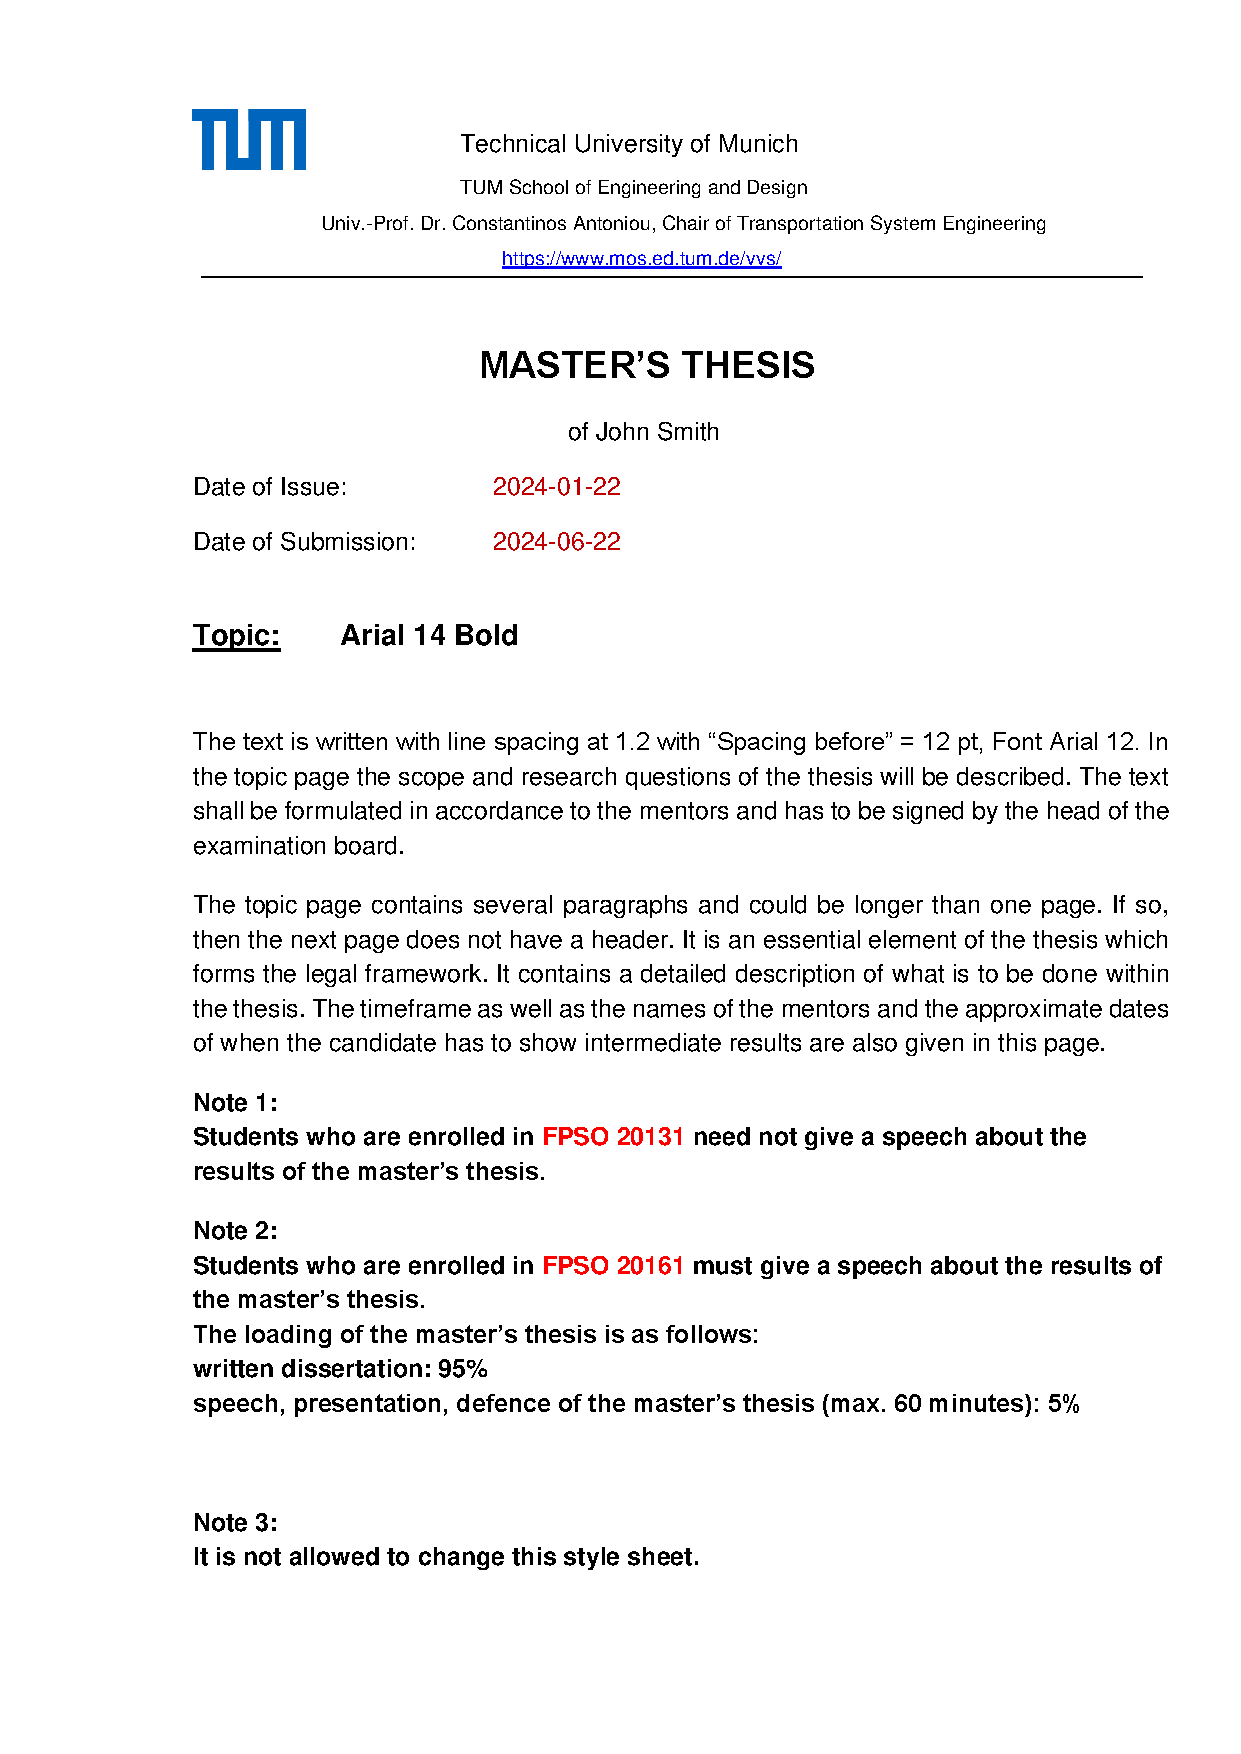
\includepdf[pages=-]{SignedTopic.pdf}%your Master Thesis Topic with Signature of Supervisor
\chapter*{\abstractname}
\thispagestyle{empty}

%TO-DO: Write your Abstract, replace random generic text
\lipsum[3]%Radom generic text




\vspace{5mm}
\textbf{Keywords:} KEYWORD1, KEYWORD2, \ldots%inserts abstract from file Abstract
\pagenumbering{Roman} %starts numbering of pages in Roman
\clearpage

\tableofcontents %inserts table of contents 
\clearpage

\setglossarystyle{long}
%TO-DO: define your acronyms here
%\newacronym{label}{acronym}{long}
\newacronym{ecb}{ECB}{European Central Bank} %first apear will be long then short onwards
\newacronym{eu}{EU}{European Union}


\setlength{\glsdescwidth}{\linewidth}  % Ensure descriptions use full line width, adjust by changing 0.8 in {0.8/linewidth} 
\printglossary[type=\acronymtype,title={List of Abbreviations},nonumberlist,style=super3col]
\clearpage

\newboldglossary{cyc}{Cycle}{A complete sequence of signal phases}
\newboldglossary{pha}{Phase}{A distinct period during which specific traffic signals are active to control vehicle and pedestrian movement.}
\printglossary[nonumberlist]
\clearpage

\addcontentsline{toc}{chapter}{List of Symbols} 
\chapter*{List of Symbols}
\begin{tabbing}
\hspace{2cm} \= \hspace{3cm} \= \kill % Set tab stops

$c_0$ \> [km/h] \> Propagation speed of kinematic waves \\
$\eta_0$ \> [km/h] \> Viscosity coefficient \\
$\nu$ \> [$\text{km}^2/\text{h}$] \> Kinematic viscosity \\

\end{tabbing}
\clearpage

\addcontentsline{toc}{chapter}{List of Figures} % Adds List of Figures to Contents
\listoffigures
\clearpage

\addcontentsline{toc}{chapter}{List of Tables} 
\listoftables
\clearpage

\setcounter{page}{1}%numbering starts at 1
\pagenumbering{arabic}%main part is numbered in arabic

\includefilesfrom{Chapter}

\addcontentsline{toc}{chapter}{Bibliography}
\printbibliography

\appendix
\includefilesfrom{Appendix}

%Avoid modifying this section unless necessary

\chapter*{\vspace{-20mm} % Move the content up
\begin{flushright}
    
\includegraphics[height=15mm]{DefaultTemplate/Logos/TUM2.png}
\end{flushright}
\begin{flushleft}
    \vspace{-20mm}
    
\includegraphics[height=15mm]{DefaultTemplate/Logos/TUM-Asia.png}
\end{flushleft}
\vspace{5mm} % Adjust space after the logo
Statutory Declaration\\
\footnotesize(according to § 20 Par. 5 FPSO)}

\thispagestyle{empty}

I solemnly declare the research in the chapters of this thesis was in full my own without the use of other sources of help not mentioned or cited in this thesis and that this thesis in substantially its present form has not been submitted or accepted previously for the award of a degree or diploma in this or any other tertiary institution and is not being submitted for a degree or diploma in any other tertiary institution or for another degree or diploma at this institution.

\vspace{30mm}

\begin{tabular}{l l}
Start of Thesis:        &\getStartDate{}\\
Date of submission:     &\getSubmissionDate{}     \\
\end{tabular}

\vspace{50mm}

\noindent\rule{5cm}{.4pt}\hfill\rule{5cm}{.4pt}\par
\hspace{8mm} Date, Place \hspace{80mm} Signature

\end{document}